

\title{T-61.5130 Machine Learning and Neural Networks}
\author{Karhunen, Luttinen}
\date{Exercise 1, 4.11.2012}


\begin{document}

\maketitle

\begin{enumerate}

\item

  An odd sigmoid function is defined by
  \begin{equation*}
    \varphi(v)=\frac{1-\exp(-av)}{1+\exp(-av)}=\tanh(av/2),
  \end{equation*}
  where $\tanh$ denotes a hyperbolic tangent. The limiting values of
  this second sigmoid function are $-1$ and $+1$. Show that the derivate 
  of $\varphi(v)$ with respect to $v$ is given by
  \begin{equation*}
    \frac{d\varphi}{dv}=\frac{a}{2}(1-\varphi^2(v)).
  \end{equation*}
  What is the value of this derivate at the origin? Suppose that the
  slope parameter $a$ is made infinitely large. What is the resulting
  form of $\varphi(v)$?  
  
  \begin{solution}

    The derivative of $\varphi(v)$:
    \begin{equation}
      \begin{split}
        \frac{d\varphi}{dv}&=\frac{a\exp(-av) (1 + \exp(-av)) + a\exp(-av)
          (1 - \exp(-av))} {(1+\exp(-av))^2} \\
        &= \frac{a ( \exp(-av) + \exp(-2av) + \exp(-av) - \exp(-2av) )}{(1 +
          \exp(-av))^2} \\
        &= \frac{a}{2} \frac{(1 + \exp(-av))^2 - (1 - \exp(-av))^2}{(1 +
          \exp(-av))^2} = \frac{a}{2} ( 1 - \varphi^2(v) )
      \end{split}
    \end{equation}

    At the origin: 
    \begin{equation}
      \left.\frac{d\varphi}{dv}\right|_{v=0} = \frac{a}{2} (1 - \left(
        \frac{1 - \exp(-a * 0)}{1 + \exp(-a*0)} \right)^2 = \frac{a}{2}.
    \end{equation}
    \begin{equation}
      \mbox{When  $a$ $\rightarrow$ $\infty$,  $\varphi(v)$ $\rightarrow$} \left\{ 
        \begin{array}{rl}
          +1, &v > 0 \\
          -1, &v < 0 \\
          0, &v = 0
        \end{array} \right.
    \end{equation}

    Fig.~\ref{fig:sigmoid} shows the values of the sigmoid
    function~(\ref{eq:sigmoid}) with different values of $a$.

    \begin{figure}[h]
      \begin{center}
        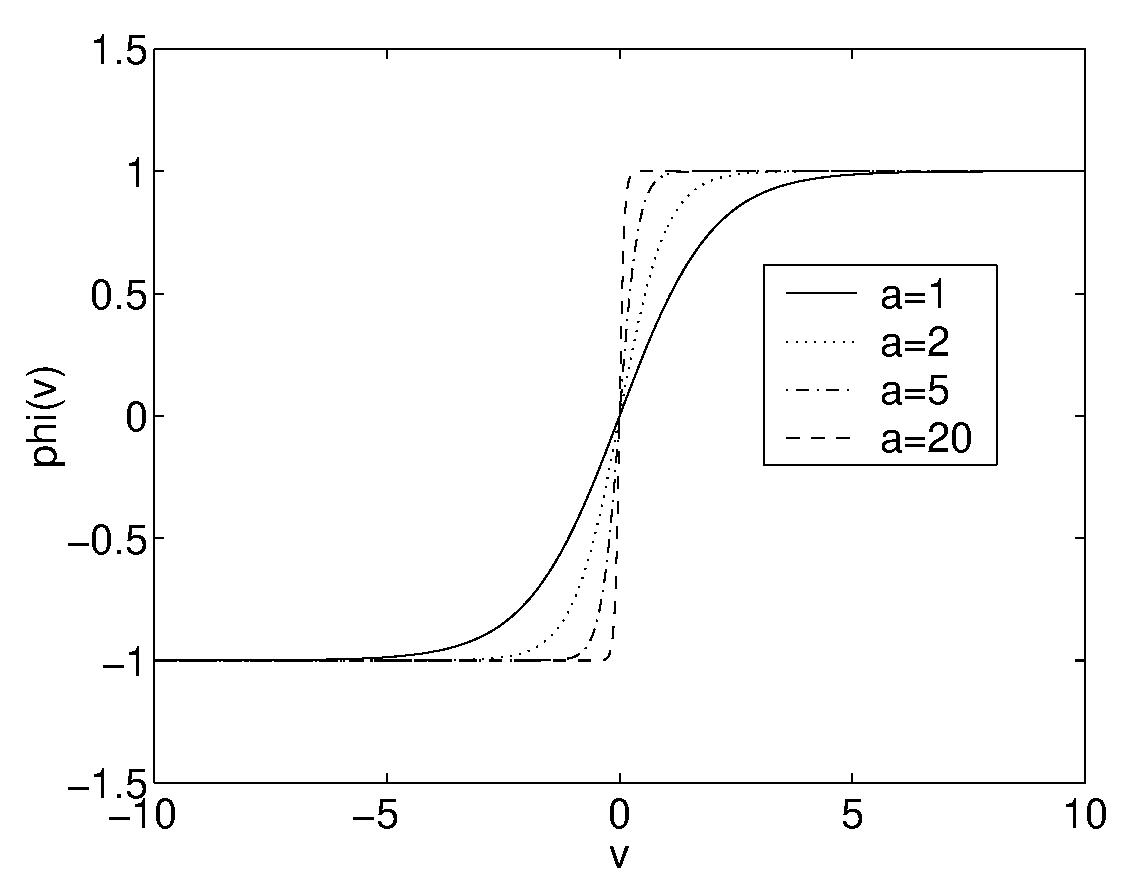
\includegraphics[width=12cm]{sigmoid.eps}
        \caption{\label{fig:sigmoid} Sigmoid function $\varphi(v)$ with
          different values of $a$. The function behaves linearly near the
          origin.}
      \end{center}
    \end{figure}

  \end{solution}
  
  
\item

  \begin{enumerate}
  \item Show that the McCulloch-Pitts formal model
    of a neuron may be approximated by a sigmoidal neuron (i.e.,
    neuron using a sigmoid activation function with large synaptic
    weights).
  \item Show that a linear neuron may be approximated by a sigmoidal
    neuron with small synaptic weights.
  \end{enumerate}
  
  \begin{solution}

    \begin{enumerate}
      
    \item The McCulloch-Pitts formula of a neuron is
      defined as a threshold function:
      \begin{equation}
        \varphi(v) = \left\{ \begin{array}{rl} 1, & v \geq 0 \\ 0, & v <
            0 \end{array} \right.,
      \end{equation}
      where $v_k = \sum_{j=1}^{m} w_{kj} x_j + b_k$, where $w_{kj}$'s are
      the synaptic weights and $b_k$ is the bias.
      
      A sigmoid activation function on interval $[0,1]$ is {\em e.g.}
      $\sigma(v) = 1 / (1 + \exp(-av))$, where we assume $a > 0$ without
      loss of generality.
      
      When synaptic weights have large values, also $|a v|$ tends to have
      a large value:
      \begin{equation}
        \begin{aligned}
          \lim_{a \rightarrow \infty} \sigma(v)& = \left. \frac{1}{1 +
              \exp(-av)}\right|_{a \rightarrow \infty} = \frac{1}{1+0} = 1 \mbox{\ \ \ \ \ \ ($v>0$)}
          \\
          \lim_{a \rightarrow \infty} \sigma(v)& = \left. \frac{1}{1 +
              \exp(-av)}\right|_{a \rightarrow \infty} =
          \frac{1}{1-\infty} = 0 \mbox{\ \ \ \ \ ($v<0$)}
        \end{aligned}
      \end{equation}
      
    \item We expand the $\exp(-av)$ in Taylor series around point $v=0$:
      
      \begin{equation}
        \begin{split}
          \sigma(v) &= \frac{1}{1 + \exp(-av)} = \frac{1}{1 + 1 - av +
            \underbrace{\frac{(av)^2}{2!} - \frac{(av)^3}{3!} +
              \cdots}_{\mbox{$\approx$ $0$, for small values of $v$}}} \\ 
          &\approx \frac{1}{2 ( 1 - \frac{av}{2})} \\
          &= \frac{1}{2} \frac{1 + \frac{av}{2}} {1 -
            \underbrace{\frac{(av)^2}{4}}_{\approx 0}} \approx \frac{1}{2}
          \left(1 + \frac{av}{2} \right) = L(v) \: _\Box
        \end{split}
      \end{equation}
      
    \end{enumerate}

  \end{solution}
  

\item

  Consider a multilayer feedforward network, all the neurons of which
  operate in their linear regions. Justify the statement that such a
  network is equivalent to a single-layer feedforward network.

  \begin{solution}
    A single neuron is depicted in Fig.~\ref{fig:singleneuron}


    \begin{figure}[hb]
      \begin{center}
        % use '../process_fig.sh neuron.fig' to make the .pstex_t
        \input neuron.pstex_t
        \caption{\label{fig:singleneuron} A single sigmoidal neuron.}
      \end{center}
    \end{figure}
    
    There the input $v_k$ to the nonlinearity $\varphi$ is defined as
    $v_k = \sum_{j = 0}^n w_{kj}x_j = \vect{w}_k^T \vect{x}$, \newline
    where $\vect{x}=\begin{pmatrix} 1 & x_1 &\cdots & x_n
    \end{pmatrix}^T$ and $\vect{w}_k=\begin{pmatrix} w_{k0} &\cdots &
      w_{kn} \end{pmatrix}^T$.

    When the neuron operates in its linear region, $\varphi(v) \approx
    \alpha v$ and $y_k \approx \alpha \vect{w}_k^T \vect{x}$. For the
    whole layer, this gives: 

    \begin{equation}
      \vect{y} = \begin{pmatrix}  y_1 \\ \cdots \\ y_m \end{pmatrix}
      \approx \alpha \begin{pmatrix}  \vect{w}_1^T \vect{x}\\ \cdots \\
        \vect{w}_m^T \vect{x} \end{pmatrix} 
      = \alpha \begin{pmatrix}  \vect{w}_1^T\\ \cdots \\
        \vect{w}_m^T \end{pmatrix} \vect{x} = \matr{W} \vect{x},
    \end{equation}
    where
    \begin{equation}
      \matr{W} = \alpha \begin{pmatrix}
        w_{10} & \cdots & w_{1n} \\ \vdots & \ddots & \vdots \\
        w_{m0} & \cdots & w_{mn} 
      \end{pmatrix}
    \end{equation}
    
    The whole network is constructed from these single layers:

    \begin{center}
      % use '../process_fig.sh network.fig' to make the .pstex_t
      \input network.pstex_t
    \end{center}
    
    and the output of the whole network is

    \begin{equation}
      \vect{y} = \matr{W_N} \vect{u_{N-1}} = \matr{W_N}  \matr{W_{N-1}}
      \vect{u_{N-2}} = \prod_{i = 1}^{N} \matr{W_i} \vect{x}.
    \end{equation}

    The product $\matr{T} = \prod_{i = 1}^{N} \matr{W_i}$ is a matrix of
    size $m \times n$: 

    \begin{equation}
      \vect{y} = \matr{T} \vect{x} = 
      \begin{pmatrix}
        t_{10} & \cdots & t_{1n} \\ \vdots & \ddots & \vdots \\
        t_{m0} & \cdots & t_{mn} 
      \end{pmatrix} \vect{x} = 
      \begin{pmatrix}  \vect{t}_1^T\\ \cdots \\
        \vect{t}_m^T 
      \end{pmatrix} \vect{x},
    \end{equation}
    
    which is exactly the output of a single layer linear network having
    $\matr{T}$ as the weights $_\Box$

  \end{solution}
  
\item

  \begin{enumerate}
  \item Construct a recurrent neural network which has two neurons in
    the input layer plus bias terms, and 3 neurons in the hidden layer
    having recurrent connections with self-feedback.  The output of
    the network is the output of the first hidden neuron.
  \item Write the equations describing the operation of this network.
  \end{enumerate}

  \begin{solution}
  \end{solution}
  
\end{enumerate}





\end{document}             % End of document.
